% !TEX program = pdflatex
% NetFRAME Home Lab — Network Topology & Systems Reference
% Build:  latexmk -pdf NetFRAME-Network-Topology.tex   (or: pdflatex twice)
% Requires: texlive-latex-recommended texlive-pictures texlive-latex-extra texlive-fonts-recommended
\documentclass[11pt,a4paper]{article}

\usepackage[T1]{fontenc}
\usepackage[utf8]{inputenc}
\usepackage{lmodern}
\usepackage[margin=2cm,headheight=15pt]{geometry}
\usepackage{xcolor}
\usepackage{graphicx}
\usepackage{booktabs}
\usepackage{longtable}
\usepackage{array}
\usepackage{tabularx}
\usepackage{amssymb}
\usepackage{enumitem}
\usepackage{fancyhdr}
\usepackage{titlesec}
\usepackage[most]{tcolorbox}
\usepackage{tikz}
\usetikzlibrary{positioning,shapes.geometric,arrows.meta,calc,backgrounds,fit,shadows.blur}
\usepackage[hidelinks,colorlinks=true,linkcolor=nfblue,urlcolor=nfgreen]{hyperref}

% ---- Palette ----
\definecolor{nfink}{HTML}{12131A}
\definecolor{nfblue}{HTML}{2B5EA8}
\definecolor{nfgreen}{HTML}{2E7D46}
\definecolor{nfviolet}{HTML}{6B4F9E}
\definecolor{nfamber}{HTML}{C8871B}
\definecolor{nfred}{HTML}{B4322B}
\definecolor{nforange}{HTML}{CC5522}
\definecolor{nfslate}{HTML}{3A4150}
\definecolor{nfgrey}{HTML}{EDEFF3}
\definecolor{nfgrey2}{HTML}{DDE2EA}

% ---- Header / footer ----
\pagestyle{fancy}
\fancyhf{}
\lhead{\small\textsc{NetFRAME Network Topology Reference}}
\rhead{\small v1.0 · 2026-07-08}
\lfoot{\small Sanitized public edition}
\rfoot{\small\thepage}
\renewcommand{\headrulewidth}{0.4pt}

% ---- Section styling ----
\titleformat{\section}{\Large\bfseries\color{nfink}}{\thesection}{0.6em}{}[{\color{nfblue}\titlerule[1.2pt]}]
\titleformat{\subsection}{\large\bfseries\color{nfslate}}{\thesubsection}{0.5em}{}

% ---- Callout boxes ----
\newtcolorbox{finding}[1][]{colback=nfred!6,colframe=nfred,boxrule=0.8pt,left=6pt,right=6pt,top=4pt,bottom=4pt,fonttitle=\bfseries,title={#1}}
\newtcolorbox{wow}[1][]{colback=nfgreen!6,colframe=nfgreen,boxrule=0.8pt,left=6pt,right=6pt,top=4pt,bottom=4pt,fonttitle=\bfseries,title={#1}}
\newtcolorbox{note}[1][]{colback=nfblue!6,colframe=nfblue,boxrule=0.8pt,left=6pt,right=6pt,top=4pt,bottom=4pt,fonttitle=\bfseries,title={#1}}

\newcommand{\ip}[1]{\texttt{#1}}
\renewcommand{\arraystretch}{1.25}

% ---- TikZ styles ----
\tikzset{
  dev/.style={draw=nfslate,fill=nfgrey,rounded corners=2pt,minimum height=8mm,minimum width=22mm,font=\footnotesize,align=center,blur shadow={shadow blur steps=5,shadow xshift=0.4pt,shadow yshift=-0.4pt}},
  net/.style={dev,fill=nfink,text=white,draw=nfink},
  fw/.style={dev,fill=nfgreen!20,draw=nfgreen},
  node730/.style={dev,fill=nfred!14,draw=nfred},
  small/.style={dev,fill=nfblue!12,draw=nfblue},
  stor/.style={dev,fill=nfamber!16,draw=nfamber},
  vlanpill/.style={rounded corners=3pt,draw,font=\scriptsize\bfseries,inner sep=2pt,minimum width=14mm,text=white},
  lnk/.style={-{Latex[length=2mm]},thick,draw=nfslate},
  lnk10/.style={-{Latex[length=2mm]},very thick,draw=nfgreen},
}

\begin{document}

% ============================ TITLE PAGE ============================
\begin{titlepage}
\thispagestyle{empty}
\begin{tikzpicture}[remember picture,overlay]
  \fill[nfink] (current page.north west) rectangle ([yshift=-6.2cm]current page.north east);
  \node[anchor=west,text=white,font=\Huge\bfseries] at ([xshift=2cm,yshift=-2.6cm]current page.north west) {NetFRAME};
  \node[anchor=west,text=nfgrey2,font=\LARGE] at ([xshift=2cm,yshift=-3.7cm]current page.north west) {Network Topology \& Systems Reference};
  \node[anchor=west,text=nfgreen,font=\large\ttfamily] at ([xshift=2cm,yshift=-4.7cm]current page.north west) {192.168.10.0/24 · km-cluster · 7 nodes · 3 GPUs · 4× RAIDZ2};
\end{tikzpicture}
\vspace{7cm}

\noindent\begin{tabularx}{\textwidth}{@{}l X@{}}
\toprule
\textbf{Owner} & Kyle Mason (\texttt{machismo0311}) — Greater Cleveland, OH \\
\textbf{Document} & NetFRAME Network Topology \& Systems Reference \\
\textbf{Version} & 1.0 \\
\textbf{Generated} & 2026-07-08 \\
\textbf{Classification} & Public / Sanitized (service tags \& serials omitted) \\
\textbf{Method} & Live discovery (nmap · Proxmox API · SSH facts · Headscale · ZFS) reconciled against the Home-Lab vault \\
\textbf{Scope} & Every host, VLAN, subnet, link, service, pool, and overlay path \\
\bottomrule
\end{tabularx}

\vfill
\begin{center}\small\color{nfslate}
Single-site production-grade home lab · Proxmox VE 9.2.3 · Juniper-cored VLAN fabric · ZFS + PBS · private GPU LLM platform
\end{center}
\end{titlepage}

\tableofcontents
\newpage

% ============================ 1. SUMMARY ============================
\section{Executive Summary}
\textbf{NetFRAME} is a single-site, 42U home lab built around a \textbf{7-node Proxmox VE 9.2.3 cluster} (\texttt{km-cluster}), a \textbf{Juniper-cored, VLAN-segmented fabric}, and a \textbf{24-bay ZFS storage node} providing NFS and Proxmox Backup Server. It runs reverse-proxied web services with automated TLS, a Prometheus/Grafana/Loki observability stack, drive-health telemetry across \textasciitilde50 disks, a Wazuh SIEM, an internal ACME PKI, a password vault, and a \textbf{GPU-accelerated private LLM platform} (RTX 8000 + dual RTX 6000, \textasciitilde96\,GB VRAM) with a custom OpenAI-compatible router that transparently escalates to the Claude API.

\vspace{2mm}
\noindent\begin{tabularx}{\textwidth}{@{}Xr@{\hskip 2em}Xr@{}}
\toprule
Proxmox nodes (quorate) & 7/7 & ZFS raw / usable & 36.7\,TB / \textasciitilde23\,TB \\
Standalone hypervisor & 1 (pve1) & PBS datastore & 24.6\,TB \\
VMs / LXCs & 2 / 6 & Monitored drives & \textasciitilde50 \\
Managed switches & 3 & Overlay VPN nodes & 9 \\
VLANs defined & 7 & Aggregate RAM & \textasciitilde1.5\,TB \\
Physical GPUs / VRAM & 3 / \textasciitilde96\,GB & UPS (split-bus) & 2 / \textasciitilde2220\,W \\
\bottomrule
\end{tabularx}

\begin{note}[Edge model — deliberate double-NAT]
A UniFi Dream Router is the WAN edge (\ip{192.168.1.0/24}); \textbf{OPNsense} (VM 100 on \texttt{pve2}) is the LAN router / firewall / DHCP for \ip{192.168.10.0/24} and the inter-VLAN gateway. The lab LAN therefore sits behind its own firewall boundary.
\end{note}

% ============================ 2. TOPOLOGY DIAGRAM ============================
\section{Physical \& Logical Topology}
\begin{center}
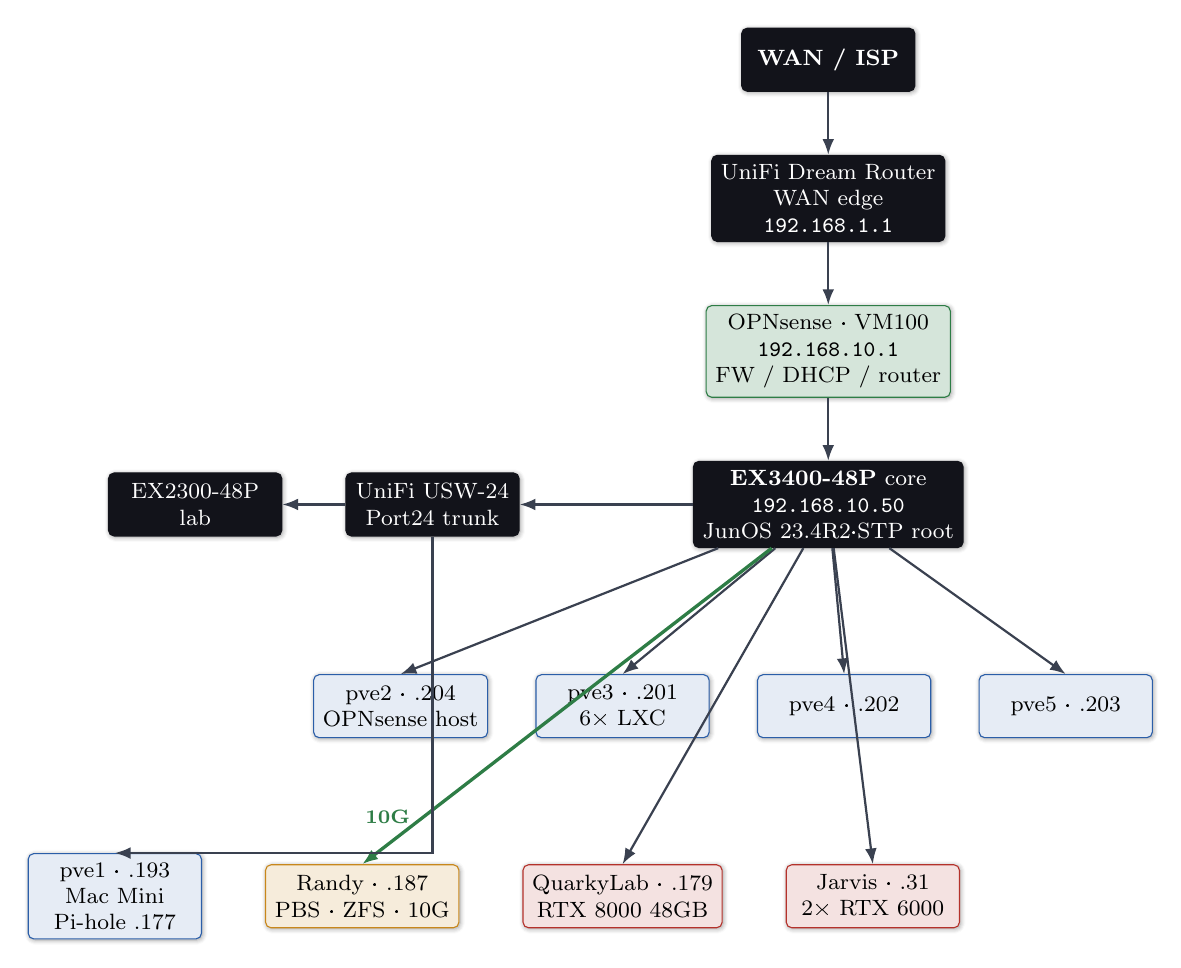
\begin{tikzpicture}[node distance=8mm and 12mm]
  \node[net] (wan) {\textbf{WAN / ISP}};
  \node[net,below=of wan] (udr) {UniFi Dream Router\\WAN edge\\\ip{192.168.1.1}};
  \node[fw,below=of udr] (opn) {OPNsense · VM100\\\ip{192.168.10.1}\\FW / DHCP / router};
  \node[net,below=of opn] (ex34) {\textbf{EX3400-48P} core\\\ip{192.168.10.50}\\JunOS 23.4R2·STP root};

  \node[net,left=22mm of ex34] (usw) {UniFi USW-24\\Port24 trunk};
  \node[net,left=8mm of usw] (ex23) {EX2300-48P\\lab};

  % compute row
  \node[small,below left=16mm and 26mm of ex34] (pve2) {pve2 · .204\\OPNsense host};
  \node[small,right=6mm of pve2] (pve3) {pve3 · .201\\6× LXC};
  \node[small,right=6mm of pve3] (pve4) {pve4 · .202};
  \node[small,right=6mm of pve4] (pve5) {pve5 · .203};

  \node[node730,below=16mm of pve3] (quark) {QuarkyLab · .179\\RTX 8000 48GB};
  \node[node730,right=8mm of quark] (jarvis) {Jarvis · .31\\2× RTX 6000};
  \node[stor,left=8mm of quark] (randy) {Randy · .187\\PBS · ZFS · 10G};
  \node[small,left=8mm of randy] (pve1) {pve1 · .193\\Mac Mini\\Pi-hole .177};

  \draw[lnk] (wan)--(udr); \draw[lnk] (udr)--(opn); \draw[lnk] (opn)--(ex34);
  \draw[lnk] (ex34)--(usw); \draw[lnk] (usw)--(ex23);
  \draw[lnk] (ex34)-- (pve2.north); \draw[lnk] (ex34)--(pve3.north);
  \draw[lnk] (ex34)--(pve4.north); \draw[lnk] (ex34)--(pve5.north);
  \draw[lnk] (ex34)--(quark.north); \draw[lnk] (ex34)--(jarvis.north);
  \draw[lnk10] (ex34)--(randy.north) node[pos=0.85,left=1pt,font=\scriptsize\bfseries,text=nfgreen] {10G};
  \draw[lnk] (usw)|-(pve1.north);
\end{tikzpicture}
\end{center}
\begin{center}\footnotesize Thick green = 10\,GbE (Randy \ip{xe-0/2/0}; Jarvis \ip{xe-0/2/2}). All other links 1\,GbE. \end{center}

% ============================ 3. L1 PHYSICAL ============================
\section{Layer 1 — Physical}
\subsection{Rack elevation (NetFRAME CS9000, 42U — rear panel removed for R730 depth)}
\begin{center}
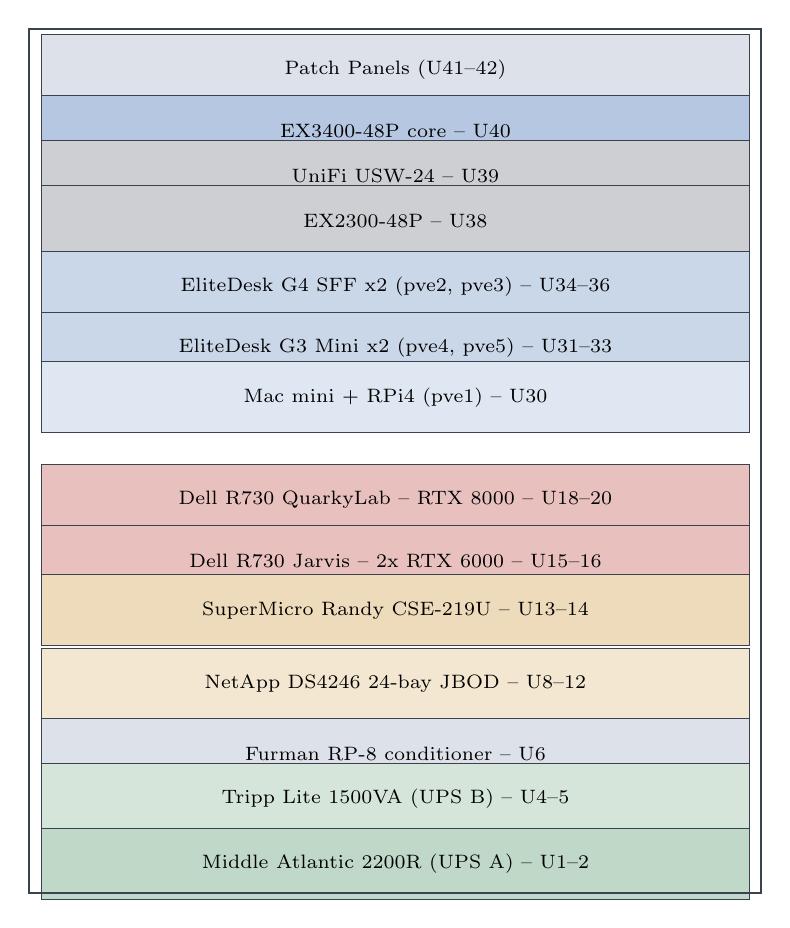
\begin{tikzpicture}[x=1cm,y=0.52cm]
  \def\w{9}
  \foreach \y/\c/\lab in {
    20/nfgrey2/{Patch Panels (U41--42)},
    18.5/nfblue!35/{EX3400-48P core -- U40},
    17.4/nfslate!25/{UniFi USW-24 -- U39},
    16.3/nfslate!25/{EX2300-48P -- U38},
    14.7/nfblue!25/{EliteDesk G4 SFF x2 (pve2, pve3) -- U34--36},
    13.2/nfblue!25/{EliteDesk G3 Mini x2 (pve4, pve5) -- U31--33},
    12/nfblue!15/{Mac mini + RPi4 (pve1) -- U30},
    9.5/nfred!30/{Dell R730 QuarkyLab -- RTX 8000 -- U18--20},
    8/nfred!30/{Dell R730 Jarvis -- 2x RTX 6000 -- U15--16},
    6.8/nfamber!30/{SuperMicro Randy CSE-219U -- U13--14},
    5/nfamber!20/{NetApp DS4246 24-bay JBOD -- U8--12},
    3.3/nfgrey2/{Furman RP-8 conditioner -- U6},
    2.2/nfgreen!20/{Tripp Lite 1500VA (UPS B) -- U4--5},
    0.6/nfgreen!30/{Middle Atlantic 2200R (UPS A) -- U1--2}}
    {\node[draw=nfslate,fill=\c,minimum width=\w cm,minimum height=0.9cm,font=\scriptsize,anchor=west] at (0,\y) {\lab};}
  \draw[nfslate,thick] (-0.15,-0.1) rectangle (\w+0.15,21);
\end{tikzpicture}
\end{center}

\subsection{Key physical links}
\begin{center}\footnotesize
\begin{tabularx}{\textwidth}{@{}l l l l X@{}}
\toprule
From & Port & To & Speed & Notes \\ \midrule
EX3400 & \texttt{ge-0/0/46} & UniFi USW-24 P24 & 1G & 802.1Q trunk (native 1 + tagged 20/30/40/50/60/70) \\
EX3400 & \texttt{ge-0/0/45} & EX2300 & 1G & Trunk, all VLANs \\
EX3400 & \texttt{xe-0/2/0} & Randy nic3 (Mellanox) & \textbf{10G} & Storage / NFS data path \\
EX3400 & \texttt{xe-0/2/2} & Jarvis enp132s0 (ConnectX) & \textbf{10G} & Access VLAN 30 \\
EX3400 & \texttt{ge-0/0/24} & QuarkyLab nic2 & 1G & Trunk native 1 + tagged 30 \\
EX3400 & \texttt{ge-0/0/22} & Jarvis nic2 & 1G & Native VLAN 1 (mgmt/corosync) \\
EX3400 & \texttt{ge-0/0/30·32·44} & iDRAC/IPMI OOB & 1G & Tagged VLAN 20 only \\
EX3400 & \texttt{xe-0/2/3} & UniFi SFP2 DAC & --- & \textbf{DOWN} — 10G/1G EEPROM mismatch \\
\bottomrule
\end{tabularx}
\end{center}

\subsection{Power — split-bus one-line}
\begin{center}
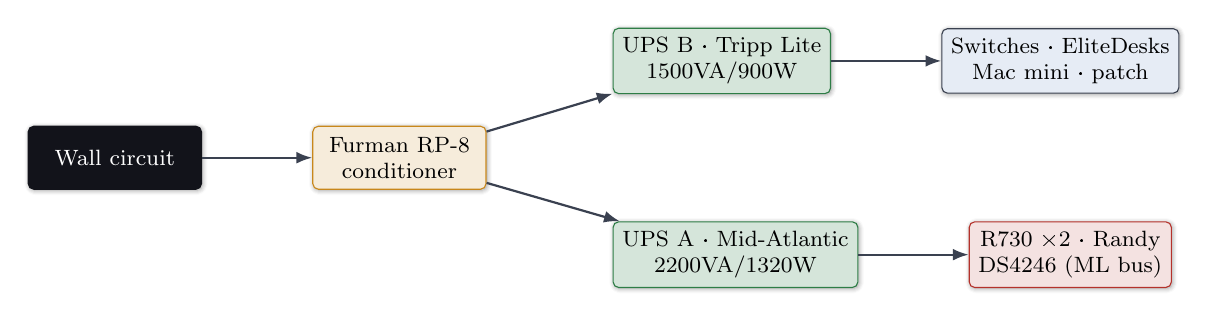
\begin{tikzpicture}[node distance=6mm and 14mm]
  \node[net] (wall) {Wall circuit};
  \node[stor,right=of wall] (furman) {Furman RP-8\\conditioner};
  \node[fw,above right=4mm and 16mm of furman] (upsb) {UPS B · Tripp Lite\\1500VA/900W};
  \node[fw,below right=4mm and 16mm of furman] (upsa) {UPS A · Mid-Atlantic\\2200VA/1320W};
  \node[dev,right=of upsb,fill=nfblue!12] (loadb) {Switches · EliteDesks\\Mac mini · patch};
  \node[node730,right=of upsa] (loada) {R730 ×2 · Randy\\DS4246 (ML bus)};
  \draw[lnk](wall)--(furman); \draw[lnk](furman)--(upsb);\draw[lnk](furman)--(upsa);
  \draw[lnk](upsb)--(loadb);\draw[lnk](upsa)--(loada);
\end{tikzpicture}
\end{center}
\begin{finding}[Capacity watch]
UPS A carries both GPU R730s. RTX 8000 alone can draw \textasciitilde260\,W under CUDA; with Jarvis's 2× RTX 6000 online, full ML load approaches the 1320\,W continuous rating. Both UPS units are exposed via \textbf{NUT 2.8.1} on \texttt{pve3:3493} (UPS A over SNMP card \ip{192.168.10.180}, UPS B over USB).
\end{finding}

% ============================ 4. L2 ============================
\section{Layer 2 — Switching \& VLANs}
\subsection{Switch fabric}
\begin{center}\footnotesize
\begin{tabularx}{\textwidth}{@{}l l l X@{}}
\toprule
Device & Mgmt IP & OS & Role \\ \midrule
EX3400-48P & \ip{192.168.10.50} & JunOS 23.4R2-S7.4 & \textbf{Core} — 48×1G PoE+, 4×10G SFP+, 2×40G QSFP+, dual PSU, STP root (prio 4096) \\
UniFi USW-24-250W & UniFi-managed & UniFi & Access / AP aggregation; Port 24 trunk \\
EX2300-48P & via trunk & JunOS & Secondary / lab isolation \\
UniFi Dream Router & \ip{192.168.1.1} & UniFi & WAN edge (upstream of OPNsense) \\
\bottomrule
\end{tabularx}
\end{center}

\subsection{VLAN matrix}
\begin{center}
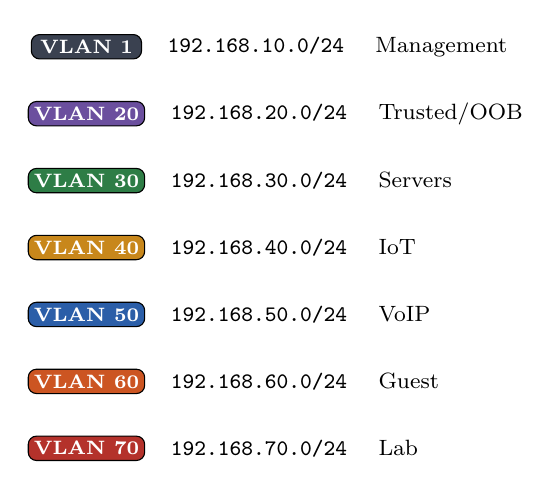
\begin{tikzpicture}[node distance=3mm]
  \foreach \i/\id/\net/\c/\lab in {0/1/{192.168.10.0/24}/nfslate/Management,1/20/{192.168.20.0/24}/nfviolet/{Trusted/OOB},2/30/{192.168.30.0/24}/nfgreen/Servers,3/40/{192.168.40.0/24}/nfamber/IoT,4/50/{192.168.50.0/24}/nfblue/VoIP,5/60/{192.168.60.0/24}/nforange/Guest,6/70/{192.168.70.0/24}/nfred/Lab}
  {\node[vlanpill,fill=\c] (v\i) at (0,-\i*0.85) {VLAN \id};
   \node[right=2mm of v\i,font=\footnotesize] {\texttt{\net} \quad \lab};}
\end{tikzpicture}
\end{center}
Gateways are OPNsense SVIs (\ip{192.168.X.1}); EX3400 carries the L3 mgmt SVI on \texttt{irb.10}.
\begin{note}[JunOS ELS gotcha (live)]
On this EX3400, \texttt{native-vlan-id} must be set at the \textbf{physical-interface} level, \emph{not} under \texttt{unit 0 family ethernet-switching}. Misplacement previously caused a trunk outage. The tagged trunk to UniFi is \texttt{ge-0/0/46}.
\end{note}

% ============================ 5. L3 ============================
\section{Layer 3 — Addressing, Routing, DNS}
\subsection{Static IP registry (VLAN 1)}
\begin{center}\footnotesize
\begin{longtable}{@{}l l p{11cm}@{}}
\toprule IP & Host & Role \\ \midrule \endhead
\ip{.1} & OPNsense & LAN gateway / FW / DHCP (VM100, pve2) \\
\ip{.2} & UniFi USW-24 & Access switch mgmt \\
\ip{.31} & Jarvis & R730 LLM node \\
\ip{.50} & EX3400 & Core switch \\
\ip{.100/.199} & Ares & Admin workstation (wired / WiFi) \\
\ip{.148} & Homepage & LXC 106 \\
\ip{.177} & Pi-hole & LXC 103 on pve1 (Mac Mini) \\
\ip{.179} & QuarkyLab & R730 ML node \\
\ip{.180} & UPS A SNMP & Mid-Atlantic OL2200R card \\
\ip{.181} & Nginx Proxy Mgr & LXC 101 \\
\ip{.182} & Vaultwarden & LXC 102 \\
\ip{.183} & Grafana/Prom/Loki/Influx/Scrutiny & LXC 103 \\
\ip{.184} & Wazuh SIEM & VM 104 (QuarkyLab) \\
\ip{.185} & Open WebUI & LXC 107 \\
\ip{.186} & Headscale & LXC 105 \\
\ip{.187} & Randy & PBS / ZFS / Jellyfin \\
\ip{.193} & pve1 & Mac Mini standalone (Pi-hole host) \\
\ip{.201--.204} & pve3/pve4/pve5/pve2 & Cluster nodes \\
\bottomrule
\end{longtable}
\end{center}

\subsection{Routing — per-node default gateway (live)}
\begin{center}\footnotesize
\begin{tabularx}{\textwidth}{@{}l l l X@{}}
\toprule Node & Default GW & Iface & Note \\ \midrule
pve2 & \ip{192.168.10.1} & vmbr1 & correct (OPNsense) \\
pve3/4/5 & \ip{192.168.1.1} & vmbr0 & \textbf{onlink to UDR — off-subnet} (finding F-1) \\
QuarkyLab & \ip{192.168.30.1} & vmbr0.30 & VLAN 30 egress \\
Jarvis & \ip{192.168.30.1} & vmbr1 & VLAN 30 egress (10G) \\
Randy & \ip{192.168.30.1} & vmbr0.30 & VLAN 30 egress \\
\bottomrule
\end{tabularx}
\end{center}

\subsection{DNS \& OOB / Servers VLANs}
Pi-hole (\ip{192.168.10.177}, FTL v6, LXC on pve1) is the LAN resolver + ad/tracker sink and serves \texttt{*.netframe.local} (e.g.\ \texttt{llm.}/\texttt{chat.}\ $\rightarrow$ NPM \ip{.181}). Public \texttt{*.kylemason.org} resolves via Cloudflare (grey-cloud) to NPM.
\begin{center}\footnotesize
\begin{tabularx}{\textwidth}{@{}l l X@{}}
\toprule IP & Host & Note \\ \midrule
\ip{192.168.20.20/21/22} & QuarkyLab iDRAC / Jarvis iDRAC / Randy IPMI & OOB VLAN 20 (2026-07-03); credentials rotated \\
\ip{192.168.30.179/187/31} & QuarkyLab / Randy / Jarvis & NFS / PBS / egress (dual-homed) \\
\bottomrule
\end{tabularx}
\end{center}

% ============================ 6. OVERLAY ============================
\section{Overlay — Headscale Mesh VPN}
Self-hosted Headscale v0.29.1 (LXC 105, \ip{192.168.10.186:8080}), tailnet \ip{100.64.0.0/10}.
\begin{center}\footnotesize
\begin{tabularx}{\textwidth}{@{}l l l l@{}}
\toprule Tailnet IP & Node & State & \phantom{x} \\ \midrule
\ip{100.64.0.1} Ares (offline) & \ip{100.64.0.2} Randy & \ip{100.64.0.3} pve5 & \ip{100.64.0.4} pve4 \\
\ip{100.64.0.5} pve3 & \ip{100.64.0.6} Jarvis & \ip{100.64.0.7} QuarkyLab & \ip{100.64.0.8} pve1 \\
\ip{100.64.0.9} Fernanda-Mac & \multicolumn{3}{l}{tag:ssh; all nodes online except laptops} \\
\bottomrule
\end{tabularx}
\end{center}

% ============================ 7. COMPUTE ============================
\section{Compute \& Virtualization — km-cluster}
\subsection{Node hardware inventory}
\begin{center}\footnotesize
\begin{tabularx}{\textwidth}{@{}l l l l l X@{}}
\toprule Node & Chassis & CPU & RAM & GPU & Kernel \\ \midrule
pve2 & EliteDesk 800 G4 & i7-8700 & 31G & --- & 7.0.12-pve \\
pve3 & EliteDesk 800 G4 & i7-8700 & 46G & --- & 7.0.12-pve \\
pve4 & EliteDesk 800 G3 Mini & i5-7500T & 31G & --- & 7.0.12-pve \\
pve5 & EliteDesk 800 G3 Mini & i5-7500T & 31G & --- & 7.0.12-pve \\
QuarkyLab & Dell R730 & 2× E5-2699v4 & 503G & RTX 8000 48G & \textbf{6.14.11-pve} \\
Jarvis & Dell R730 & 2× E5-2687Wv4 & 377G & 2× RTX 6000 & \textbf{6.14.11-pve} \\
Randy & SuperMicro CSE-219U & 2× E5-2690v4 & 125G & RX 580 & 7.0.12-pve \\
pve1 & Mac Mini (2011) & --- & --- & --- & standalone \\
\bottomrule
\end{tabularx}
\end{center}
\begin{finding}[Kernel pinning — do not upgrade]
QuarkyLab and Jarvis are pinned to \textbf{6.14.11-9-pve} via \texttt{GRUB\_DEFAULT}; 6.17+ breaks the NVIDIA 550.163.01 stack. Never run kernel upgrades or change GRUB default on either GPU node.
\end{finding}

\subsection{VM / LXC inventory}
\begin{center}\footnotesize
\begin{tabularx}{\textwidth}{@{}l l l l l X@{}}
\toprule ID & Name & Host & Res & IP & Payload \\ \midrule
VM100 & OPNsense & pve2 & 4G & \ip{.1} & LAN router/FW/DHCP v25.7 \\
VM104 & Wazuh & QuarkyLab & 16G & \ip{.184} & SIEM (no guest-agent — see §Security) \\
101 & nginx-proxy & pve3 & 512M/8G & \ip{.181} & Nginx Proxy Manager \\
102 & vaultwarden & pve3 & 512M/10G & \ip{.182} & Vaultwarden \\
103 & grafana & pve3 & 2G/20G & \ip{.183} & Grafana+Prom+Loki+Influx+Scrutiny \\
105 & headscale & pve3 & 512M/4G & \ip{.186} & Mesh VPN control \\
106 & homepage & pve3 & 512M/8G & \ip{.148} & Homepage + PeaNUT \\
107 & openwebui & pve3 & 4G/16G & \ip{.185} & Open WebUI \\
\bottomrule
\end{tabularx}
\end{center}

% ============================ 8. STORAGE ============================
\section{Storage Architecture}
\subsection{Randy ZFS \texttt{datastore} — 4× RAIDZ2 (36.7\,TB raw / \textasciitilde23\,TB usable)}
\begin{center}
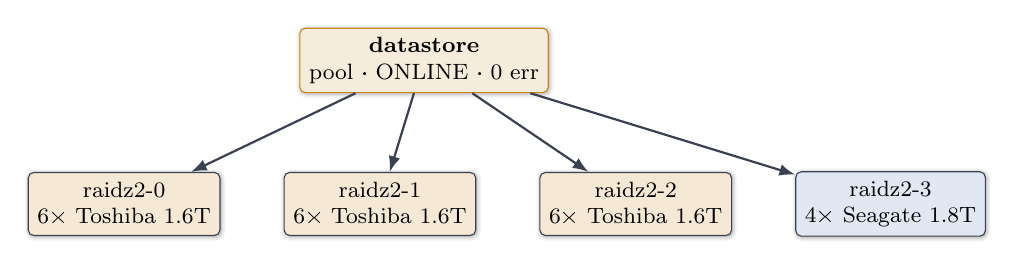
\begin{tikzpicture}[node distance=4mm and 8mm]
  \node[stor,minimum width=30mm] (pool) {\textbf{datastore}\\pool · ONLINE · 0 err};
  \node[dev,below left=10mm and 10mm of pool,fill=nfamber!18] (v0) {raidz2-0\\6× Toshiba 1.6T};
  \node[dev,right=of v0,fill=nfamber!18] (v1) {raidz2-1\\6× Toshiba 1.6T};
  \node[dev,right=of v1,fill=nfamber!18] (v2) {raidz2-2\\6× Toshiba 1.6T};
  \node[dev,right=of v2,fill=nfblue!14] (v3) {raidz2-3\\4× Seagate 1.8T};
  \draw[lnk](pool)--(v0);\draw[lnk](pool)--(v1);\draw[lnk](pool)--(v2);\draw[lnk](pool)--(v3);
\end{tikzpicture}
\end{center}
Boot: RAID-1 mirror (2× ST200FM0053 SAS) on \textbf{AVAGO 3108 MegaRAID}; data drives on a \textbf{separate LSI 9207-8e in IT mode}. PBS v4.2.2 (\ip{192.168.10.187:8007}) exposes a 24.6\,TB datastore.
\begin{wow}[Live finding — DS4246 dual-path SAS]
The NetApp DS4246 shelf's 4\,TB drives enumerate as \textbf{duplicate serial pairs} — dual-path SAS multipath through the shelf's two I/O modules presenting each disk on two paths. Configure \texttt{multipath}/dm before pooling. (This also flags drift: docs list 2\,TB drives; live shelf is 4\,TB-class, buildout in progress.)
\end{wow}
\begin{finding}[PBS storage pin (F-4, resolved)]
The VLAN-30 migration silently repointed PBS storage to \ip{.30.187} and stalled VLAN-1 node backups from 2026-07-02; fixed 2026-07-06 back to \ip{192.168.10.187}. \textbf{Keep PBS storage on \ip{.10.187}.}
\end{finding}

% ============================ 9. SERVICES ============================
\section{Services \& Application Layer}
\subsection{Reverse proxy \& published services (NPM, CT101)}
\begin{center}\footnotesize
\begin{tabularx}{\textwidth}{@{}l l l X@{}}
\toprule Hostname & Backend & TLS & Auth \\ \midrule
vault.kylemason.org & \ip{.182} & CF DNS-01 & Vaultwarden \\
grafana.kylemason.org & \ip{.183:3000} & CF DNS-01 & Grafana \\
homepage.kylemason.org & \ip{.148:3000} & CF DNS-01 & Basic (kyle) \\
wazuh.kylemason.org & \ip{.184:443} & CF DNS-01 & Wazuh \\
chat.netframe.local & Open WebUI \ip{.185} & internal & admin \\
llm.netframe.local & Jarvis \ip{.31:8000} & HTTP & Pi-hole-scoped \\
\bottomrule
\end{tabularx}
\end{center}
Observability: Prometheus (\ip{.183:9090}, localhost-only, 8 exporters), Grafana v13, Loki, InfluxDB, Scrutiny (\textasciitilde50 drives, collectors on Randy/QuarkyLab/Jarvis), NUT (\ip{pve3:3493}), CrowdSec IPS, step-ca PKI (\ip{pve2:443}).

% ============================ 10. LLM ============================
\section{AI / LLM Platform}
\begin{center}
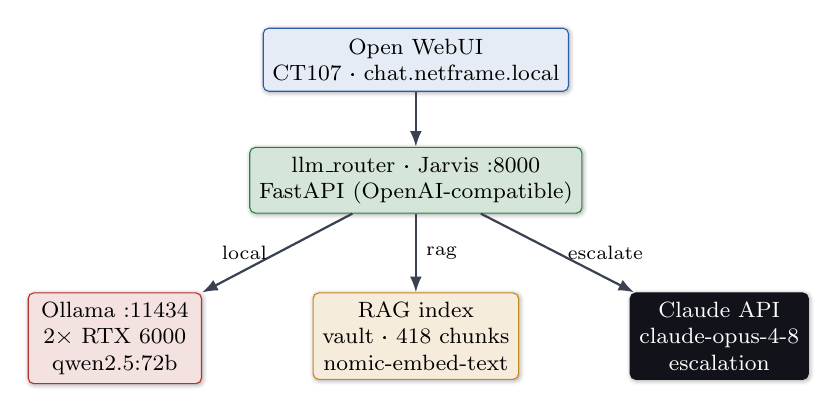
\begin{tikzpicture}[node distance=7mm and 16mm]
  \node[small] (ow) {Open WebUI\\CT107 · chat.netframe.local};
  \node[fw,below=of ow] (router) {llm\_router · Jarvis :8000\\FastAPI (OpenAI-compatible)};
  \node[node730,below left=10mm and 6mm of router] (ollama) {Ollama :11434\\2× RTX 6000\\qwen2.5:72b};
  \node[stor,below=10mm of router] (rag) {RAG index\\vault · 418 chunks\\nomic-embed-text};
  \node[net,below right=10mm and 6mm of router] (claude) {Claude API\\claude-opus-4-8\\escalation};
  \draw[lnk](ow)--(router);
  \draw[lnk](router)--(ollama) node[midway,left,font=\scriptsize] {local};
  \draw[lnk](router)--(rag) node[midway,right,font=\scriptsize] {rag};
  \draw[lnk](router)--(claude) node[midway,right,font=\scriptsize] {escalate};
\end{tikzpicture}
\end{center}
\begin{wow}[On-prem, cited answers over your own notes]
The \texttt{"rag"} model grounds answers on the Home-Lab Obsidian vault (418 chunks, cosine index) with \texttt{[source]} citations — served entirely on GPU on Jarvis, with a one-flag escalation to Claude Opus for hard queries. QuarkyLab's RTX 8000 48\,GB drives a parallel DUNE research RAG agent (Fernanda).
\end{wow}

% ============================ 11. SECURITY ============================
\section{Security Architecture}
\begin{itemize}[leftmargin=1.2em,itemsep=1pt]
  \item \textbf{OOB isolation (Phase 1):} all three BMCs moved off flat VLAN 1 onto tagged VLAN 20; default credentials rotated to Vaultwarden; reachable only from Ares \texttt{enp0s31f6.20}.
  \item \textbf{Servers VLAN 30:} GPU/storage nodes dual-homed (NFS/PBS/egress on 30; corosync/mgmt on 1).
  \item \textbf{Ingress chokepoint:} all web traffic via NPM; admin planes localhost- or Ares-bound (pentest F-03/F-05, verified).
  \item \textbf{Defense in depth:} Wazuh SIEM + CrowdSec IPS + step-ca PKI + Vaultwarden secrets.
\end{itemize}
\begin{finding}[Operational — Wazuh guest agent (F-5)]
VM 104 lacks \texttt{qemu-guest-agent}; a QuarkyLab host reboot hard-stops it and \texttt{wazuh-indexer} returns unhealthy. Recovery: \texttt{qm stop 104 \&\& qm start 104}, wait \textasciitilde4\,min (healthy = dashboard 302$\rightarrow$/login).
\end{finding}

% ============================ 12. DATA FLOWS ============================
\section{Data-Flow Walkthroughs}
\textbf{A · Grounded chat:} Browser $\to$ Pi-hole resolves \texttt{chat.netframe.local} $\to$ NPM \ip{.181} $\to$ Open WebUI \ip{.185} $\to$ \texttt{llm\_router} Jarvis \ip{.31:8000} (\texttt{rag}) $\to$ embed + cosine search vault $\to$ Ollama \texttt{qwen2.5:72b} tensor-split $\to$ cited answer.\\[2pt]
\textbf{B · Nightly backup:} \texttt{pvescheduler} $\to$ \texttt{vzdump} (02:00 CT / 03:00 VM) $\to$ PBS \ip{192.168.10.187:8007} (VLAN 1) $\to$ prune 7d+4w.\\[2pt]
\textbf{C · Storage:} GPU nodes mount Randy NFS over \textbf{VLAN 30 10G} (\ip{.30.187}, \texttt{xe-0/2/0}); corosync stays on VLAN 1.\\[2pt]
\textbf{D · BMC access:} Ares tags VLAN 20 (\texttt{enp0s31f6.20}) $\to$ EX3400 \texttt{ge-0/0/30/32/44} $\to$ iDRAC \ip{192.168.20.20-22}.

% ============================ 13. FINDINGS ============================
\section{Observations, Drift \& Recommendations}
\begin{center}\footnotesize
\begin{tabularx}{\textwidth}{@{}l l X X@{}}
\toprule \# & Sev & Finding & Recommendation \\ \midrule
F-1 & Med & Inconsistent default GWs: pve3/4/5 via \ip{192.168.1.1} (off-subnet, bypasses OPNsense) & Repoint to \ip{192.168.10.1} or document intent \\
F-2 & Low & Ares wired mgmt leg link-down; VLAN 20 reroutes via WiFi & Restore wired leg; verify \texttt{ip route get} \\
F-3 & Med & DS4246 drift + dual-path duplicates & Configure multipath before pooling; update docs \\
F-4 & \checkmark & PBS storage was repointed to \ip{.30.187} (broke backups) & Fixed; keep on \ip{.10.187}; monitor backup age \\
F-5 & Low & Wazuh VM lacks guest-agent & Install \texttt{qemu-guest-agent}; cold start \\
F-6 & Low & \texttt{xe-0/2/3} DAC down (EEPROM mismatch) & Replace SFP or decommission \\
F-7 & Info & VLANs 40/50/60/70 lightly populated & Populate or prune \\
F-8 & Low & Amazon Echo (Alexa) on flat mgmt VLAN 1 (\ip{.112}); \texttt{:1080} SOCKS5 advertises no-auth but does \textbf{not} relay (protocol-verified) --- benign firmware artifact & Move to IoT VLAN 40 (egress-only); \textbf{scheduled to move soon} \\
\bottomrule
\end{tabularx}
\end{center}

\section{Failure-Domain / Blast-Radius}
\begin{center}\footnotesize
\begin{tabularx}{\textwidth}{@{}l X l@{}}
\toprule Component & If it fails & Mitigation \\ \midrule
pve2 (OPNsense) & No LAN routing/DHCP/inter-VLAN — whole LAN & onboot; serial-console runbook \\
pve3 (6 LXCs) & NPM/Vault/Grafana/Homepage/Headscale/OpenWebUI down & PBS backups; migratable CTs \\
Randy & Backups + GPU NFS + Jellyfin & RAIDZ2 (2-disk/vdev); split HBAs \\
EX3400 & Entire wired fabric & Dual PSU; UPS B \\
UPS A & Both R730s + Randy + DS4246 & 2200VA headroom; graceful shutdown \\
pve1 & LAN DNS / ad-block & Secondary resolver \ip{1.1.1.1} \\
Corosync & Loss of quorum & 7 votes on stable VLAN-1 L2 \\
\bottomrule
\end{tabularx}
\end{center}

\section{Appendix — Live Port / Service Scan}
\footnotesize Verified 2026-07-08 (\texttt{nmap -sT -sV}, top-200). \texttt{:9100}=node-exporter, \texttt{:3128}=Proxmox \texttt{pveproxy}. Proxmox \texttt{:8006}, PBS \texttt{:8007}, Jellyfin \texttt{:8096} are outside top-200 but known-live.
\begin{center}\footnotesize
\begin{longtable}{@{}l l p{11cm}@{}}
\toprule Host & Open ports & Identity \\ \midrule \endhead
\ip{.1} OPNsense & 53,80,443 & Unbound DNS 1.23.1 + GUI \\
\ip{.2} UniFi USW & 53,80,443,8080,8443 & dnsmasq + UniFi \\
\ip{.31} Jarvis & 22,111,3128,\textbf{8000},9100 & SSH·Proxmox·llm\_router·exporter \\
\ip{.50} EX3400 & 22,830 & SSH + NETCONF \\
\ip{.100/.199} Ares & 21,22,111,139,445,2049,9090 & FTP·Samba·NFS·Cockpit \\
\ip{.112} Amazon Echo & 1080,8888 & Alexa; non-relaying SOCKS5 handshake (F-8) \\
\ip{.148} Homepage & 22,8081 & SSH·PeaNUT \\
\ip{.177} Pi-hole & 22,53,80,443 & dnsmasq pi-hole v2.92.2 \\
\ip{.179} QuarkyLab & 22,111,3128,9100 & SSH·Proxmox·exporter \\
\ip{.180} UPS card & 22,80,443 & CyberPower \\
\ip{.181} NPM & 22,80,81,443 & OpenResty proxy \\
\ip{.182} Vaultwarden & 22,80 & Vaultwarden \\
\ip{.183} Observability & 22,3000,8080,9100 & Grafana·Scrutiny·exporter \\
\ip{.184} Wazuh & 22,443 & SIEM dashboard \\
\ip{.185} Open WebUI & 22,8080 & Chat UI \\
\ip{.186} Headscale & 22,8080 & Mesh VPN control \\
\ip{.187} Randy & 22,111,2049,3128,9100 & SSH·NFS·Proxmox·exporter (+8007/8096) \\
\ip{.201--.204} pve3/4/5/2 & 22,111,3128,9100 & nodes (.204 also 443=step-ca) \\
\bottomrule
\end{longtable}
\end{center}

\vfill
\begin{center}\small\color{nfslate}
Generated 2026-07-08 from live discovery reconciled against the NetFRAME Home-Lab vault.\\ Sanitized public edition. Sanitized edition suitable for the public repo generated alongside.
\end{center}

\end{document}
